\documentclass[12pt]{article}
\usepackage[utf8]{inputenc} % Pacote para acentuação gráfica
%\usepackage[T1]{fontenc}
\usepackage[brazil]{babel} % nomes das estruturas em pt-br
%\usepackage{hyperref}
\usepackage{csquotes} % gerenciamento de aspas
\usepackage{indentfirst} % indenta primeiro paragráfo após título
\usepackage{setspace} % pacote para alterar espaçamento entre linhas
%\setlength{\parindent}{1cm} % define o tamanho da indentação
%\setlength{\parskip}{0.3cm} % define o espaçamento vertical entre parágrafos
\usepackage[top = 2cm, left = 2cm, bottom = 2cm, right = 2cm]{geometry} % define as margens do documento
\usepackage{fancyhdr} % pacote para numeração de páginas
\usepackage{lipsum}  % Pacote para gerar texto de preenchimento
\usepackage{xcolor} % Definindo novas cores
\usepackage{graphicx} % para inserir figuras
\usepackage{float} % Força o posicionamento da figura
%\usepackage{amsmath} % Este pacote é necessário para usar símbolos matemáticos
\usepackage{gensymb} % símbolos trigonométricos
\usepackage{braket} % notações em álgebra "quântica"
\usepackage{amssymb} % Para acessar os símbolos do AMS


\definecolor{verde}{rgb}{0.25,0.5,0.35}
\definecolor{jpurple}{rgb}{0.5,0,0.35}
% Configurando layout para mostrar codigos Java
\usepackage{listings}
\lstset{
	language=Python,
	basicstyle=\ttfamily\small,
	keywordstyle=\color{jpurple}\bfseries,
	stringstyle=\color{red},
	commentstyle=\color{verde},
	morecomment=[s][\color{blue}]{/**}{*/},
	extendedchars=true,
	showspaces=false,
	showstringspaces=false,
	numbers=left,
	numberstyle=\tiny,
	breaklines=true,
	backgroundcolor=\color{cyan!10},
	breakautoindent=true,
	captionpos=b,
	xleftmargin=0pt,
	tabsize=4
}
\pagestyle{empty}

\begin{document}
	
\title{\textbf{{\Huge Notas em Computação Quântica}}} % Título
\author{\textbf{{\Large Ricardo Alvarenga}}} % Autor
\date{\textbf{{\Large 2024}}} % Data
\maketitle % Criar
\thispagestyle{empty} % oculta número da página

\begin{figure}[H]
	\centering
	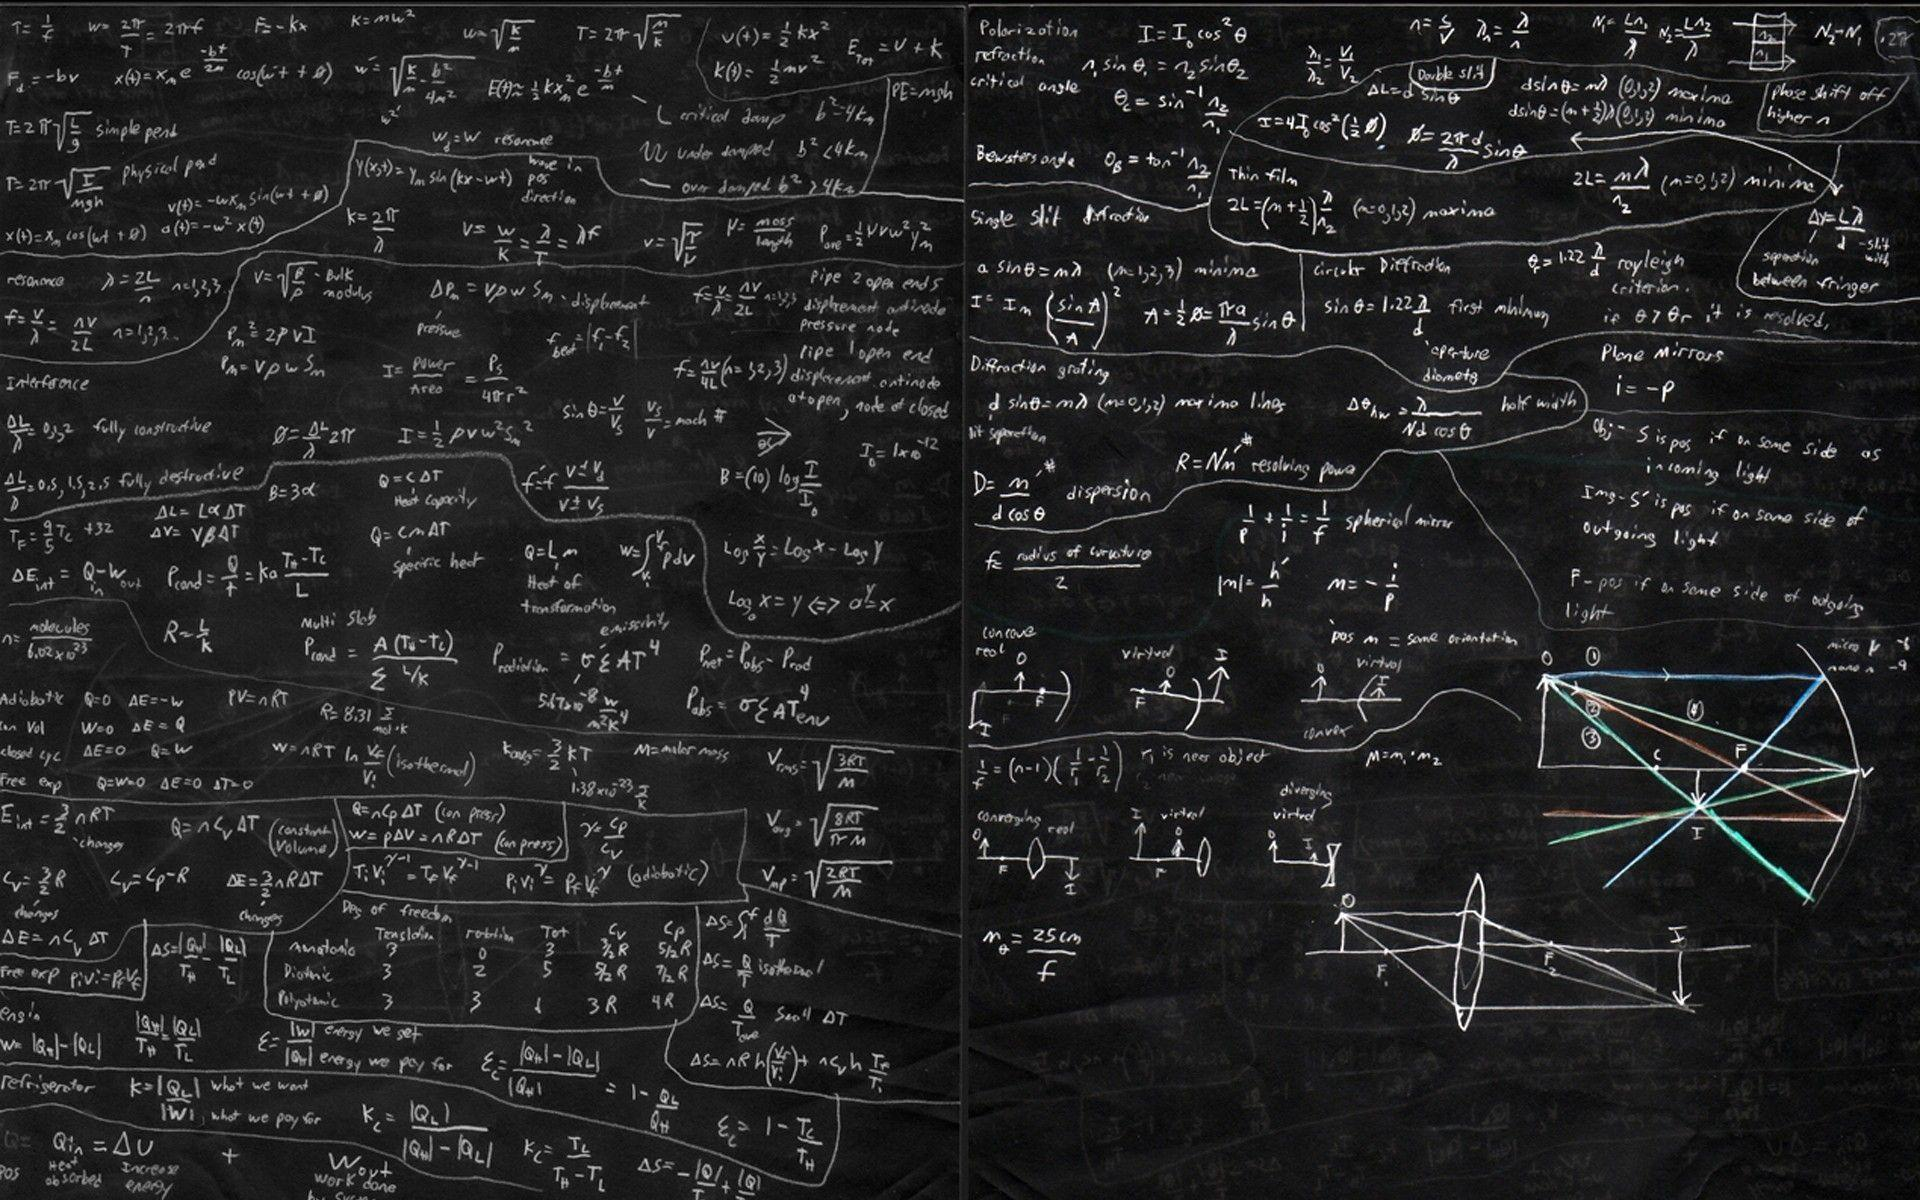
\includegraphics[width=1\linewidth]{figuras/wp5436123-quantum-physics-wallpapers}
\end{figure}


\newpage

\pagestyle{fancy}
\setcounter{page}{1} % reset contador de página
\pagenumbering{Roman}  % Altera número de página para números romanos
\tableofcontents % cria sumário
\newpage

\listoffigures % lista de figuras
\newpage


\pagestyle{fancy}
\fancyfoot[C]{\thepage} % Adiciona o número da página no centro do rodapé
\newpage

\setcounter{page}{1} % reset contador de página
\pagenumbering{arabic}
\pagestyle{fancy}
\fancyfoot[C]{\thepage}

% \twocolumn  % Inicia o ambiente de duas colunas

\onehalfspacing % espaçamento de 1,5 entre linhas

\section{Álgebra Linear}

\subsection{Vetores}

Indicaremos, nesta seção, vetores com letras minusculas em negrito \(\textbf{a, b, v, w}\) e \(\textbf{x}\), e escalares com minúsculas em itálico, como \(\textit{a, k, v, w}\) e \(\textit{x}\). Para um vetor, por exemplo, \(\textbf{v}\) com ponto inicial \(\textit{A}\) e ponto final \(\textit{B}\), usaremos\cite{anton2012algebra}: \(\textbf{v} = $\overrightarrow{\textit{AB}}$\)

Vetores são seguimentos orientados (início em 0, 0) que estão sempre no plano cartesiano. Vetores são usados para representar grandezas escalares (massa, pressão, etc.) e grandezas físicas vetoriais (velocidade, força e deslocamento).

\begin{figure}[H]
	\centering
	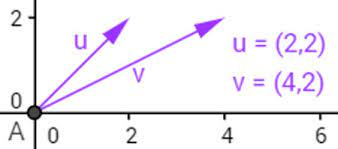
\includegraphics[width=.5\linewidth]{figuras/vetores_01}
	\caption[Vetores \textbf{u} e \textbf{v}]{Exemplos de Vetores, \(\textbf{u}\) e \(\textbf{v}\)}
	\label{fig:vetores01}
\end{figure}

\subsubsection{Vetores com duas dimensões - \(\mathbb{R}^2\)}

\(x, y\) podem assumir qualquer valor em \(\mathbb{R}\).

\begin{figure}[H]
	\centering
	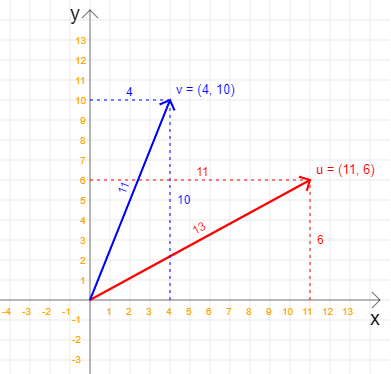
\includegraphics[height=.3\textheight]{figuras/vetores_02}
	\caption[Vetores em \( \mathbf{R}^{2} \)]{Vetores em \(\mathbb{R}^2\)}
	\label{fig:vetores02}
\end{figure}

\newpage

\subsubsection{Vetores com três dimensões -  \(\mathbb{R}^3\)}

\(x, y, z\) podem assumir qualquer valor em \(\mathbb{R}\).

\begin{figure}
	\centering
	\includegraphics[width=0.5\linewidth]{"figuras/vetores R3"}
	\caption[Vetores em \( \mathbf{R}^{3} \)]{Vetores em \(\mathbb{R}^3\)}
	\label{fig:vetores-r3}
\end{figure}

\subsubsection{Vetores com \(n\) dimensões - \(\mathbb{R}^n\)}

Os vetores com \textit{n} dimensões são de difícil (ou impossível) representação gráfica.

Um vetor \(\mathbb{R}^4\) é indicado da seguinte forma: \(\mathbb{R}^4 (x, y, z, w)\)

\subsubsection{Como plotar um vetor no plano \(\mathbb{R}^3\)}

Veja na figura \ref{fig:vetor r3} o vetor \(\textbf{u} = (2,4,3)\).

\begin{figure}
	\centering
	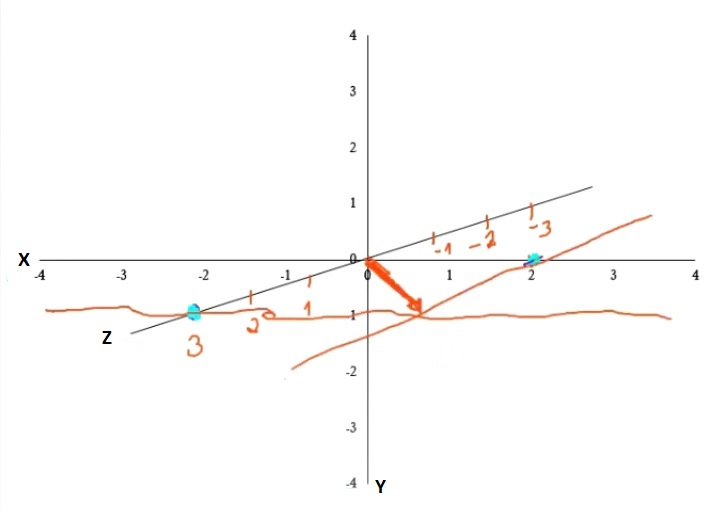
\includegraphics[width=0.7\linewidth]{figuras/R3}
	\caption[Vetor em \( \mathbf{R}^{3} \)]{Vetor em \(\mathbb{R}^3\)}
	\label{fig:vetor r3}
\end{figure}

\subsubsection{Tipos de vetores}

\singlespacing
\begin{itemize}
	\item Vetor Nulo: Todos valores iguais a zero. Ex: \(\textbf{v} = (0,0,0)\)
	\item Vetor simétrico ou oposto: Ocorre quando dois vetores são opostos e contêm o mesmo módulo e mesma direção. Ex: \(\textbf{v} = (x,y), \textbf{-v} = (-x,-y)\)
	\item Vetor unitário: Possui módulo (tamanho) igual a 1. \(|\textbf{v}| = 1\)
	\item Vetores colineares ou paralelos: Ocorrem quando dois vetores tiverem a mesma direção, na mesma reta ou retas paralelas.
	\item Vetores coplanares: Quando dois vetores fazem parte de um mesmo plano.
\end{itemize}
\onehalfspacing
\pagebreak

\subsubsection{Igualdade de vetores}

Dois vetores serão iguais se: 

\singlespacing
\begin{itemize}
	\item \(x_{1} = x_{2}\)
	\item \(y_{1} = y_{2}\)
	\item \(z_{1} = z_{2}\) vetores em \(\mathbb{R}^3\)
	\item \(w_{1} = w_{2}\) vetores em \(\mathbb{R}^4\)
\end{itemize}
\onehalfspacing

\(\textbf{u} = (3, x + 4)\) \(\textbf{v} = (3, 8)\) se \(x = 4\) os vetores serão iguais.

Sejam: \(\textbf{u} = (x-1, 3)\), \(\textbf{v} = (3, 2y-1)\). Determine o valor de \(x\) e \(y\) para que \(\textbf{u} = \textbf{v}\).

\(x = 4\), \(y = 2\)

\subsection{Componentes de um vetor}

Considere um vetor \(\textbf{v} = $\overrightarrow{P_{1}P_{2}}$\), então possui ponto inicial \(P_{1}(x_{1}, y_{1})\) e ponto final \(P_{2}(x_{2}, y_{2})\). Os componentes deste vetor são dados pela fórmula\cite{anton2012algebra}: 

\($\overrightarrow{P_{1}P_{2}}$ = (x_{2}-x_{1}, y_{2} - y_{1})\)

Que corresponde ao vetor \(\textbf{v}\) com origem em \((0, 0)\).

\subsubsection{Soma de vetores}

Para realizar a soma de dois vetores temos que efetuar a soma de cada elemento com seu correspondente.

Exemplo:

\(\textbf{u} = (2, 3)\), \(\textbf{v} = (5, 6)\)

\(\textbf{u} + v = (7, 9)\)

\subsubsection{Subtração de vetores}

\(A = (-1, 2)\)   \(B = (2,1)\). \(\textbf{v} = $\overrightarrow{AB}$\) o vetor está "perdido" no plano cartesiano. Para corrigir isso, realizamos a subtração:

\(B - A = (2, 1) - ( -1, 2) = (3, -1)\). Que resulta no vetor \(\textbf{t} = (3, -1)\), conforme figura \ref{fig:subtracaovetores01}.

Outro exemplo: Dois vetores \(\textbf{u} = (-1, 3)\) e \(\textbf{v} = (10, 20)\), a subtração \(\textbf{u} - \textbf{v}\) resulta em \((-11, -17)\).

Sejam \(\textbf{u}\) e \(\textbf{v}\) vetores no \(\mathbb{R}^n\)\cite{lipschutz-algebra}: \(\textbf{u}=(a_{1}, a_{2},...,a_{n})\) e \(\textbf{v}=(b_{1}, b_{2},...,b_{n})\)

\(\textbf{u}-\textbf{v} = (a_{1} - b_{1}, a_{2}-b_{2},...,a_{n}-b_{n})\).

\begin{figure}
	\centering
	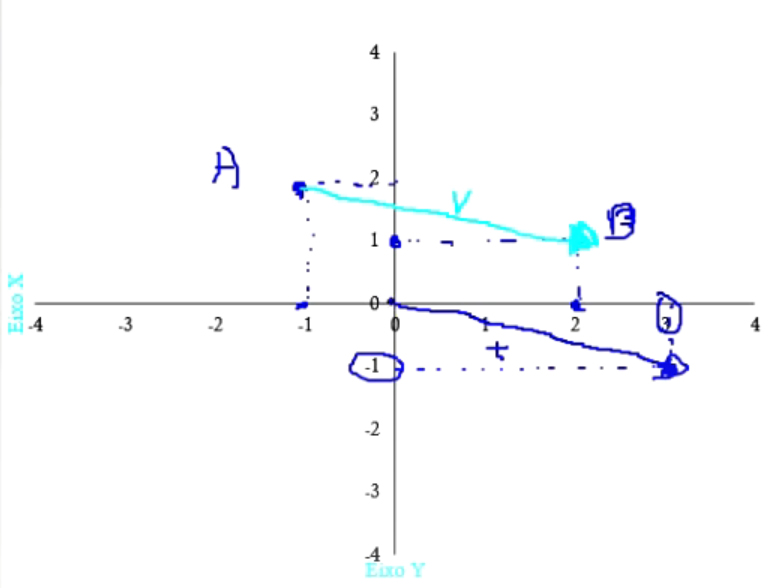
\includegraphics[width=0.7\linewidth]{figuras/subtracao_vetores_01}
	\caption[Subtração de Vetores]{Subtração de Vetores}
	\label{fig:subtracaovetores01}
\end{figure}

\subsubsection{Multiplicação de dois vetores (Produto Escalar)}

Assim como na soma e subtração de vetores, podemos multiplicar vetores. O nome correto deste tipo de operação é \textit{Produto Escalar}.

Sejam \(\textbf{u}\) e \(\textbf{v}\) vetores no \(\mathbb{R}^n\): \(\textbf{u}=(a_{1}, a_{2},...,a_{n})\) e \(\textbf{v}=(b_{1}, b_{2},...,b_{n})\)

\(\textbf{u} \cdot \textbf{v }= (a_{1} \cdot a_{2} + b_{1} \cdot b_{2} ,..., + a_{n} \cdot b_{n})\).

Exemplo: \(\textbf{u} = (1,2)\), \(\textbf{v} = (5, 3)\)
Então: \(\textbf{u} \cdot \textbf{v} = (1, 2, 3, 4) \cdot (5, 3, 1, 4) = (5 + 6 + 3 + 16) = 30\)

\subsubsection{Multiplicação por um escalar}

Multipliacação por um escalar é multiplicar um número por um vetor.

Sejam: \(\textbf{t} = (x_{1}, x_{2}, ..., x_{n})\) e um número \(\textit{a}\)

Temos: \(\textit{a}\cdot\textbf{t} = \textit{a}(x_{1}, x_{2}, ..., x_{n}) = (\textit{a} \cdot x_{1}, \textit{a} \cdot x_{2}, ..., \textit{a} \cdot x_{n})\)

Exemplo:

\(\textbf{u} = (4, 5)\) e \(\textit{a} = 2\), \(\textit{a}\cdot\textbf{u} = 2(4, 5) = (8, 10)\)

\subsubsection{Módulo/Norma (Norm) de um vetor}

A norma ou módulo de um vetor é o comprimento desse vetor, que pode ser calculado por meio da distância de seu ponto final até a origem.

A norma de \( \textbf{u} \) é denotada por \( \| \textbf{u} \| \).

Considerando o vetor \(\textbf{u} = (a_{1}, a_{2}, ..., a_{n})\), calculamos sua norma, ou módulo, da seguinte forma\cite{lipschutz-algebra, anton2012algebra}: \( \|\textbf{u}\| = \sqrt{\textbf{u} \cdot \textbf{u}} = \sqrt{a_{1}^2 + a_{2}^2 + ... + a_{n}^2} \) 

Exemplo: \(\textbf{v} = (5, 6)\), \(\|\textbf{v}\| = \sqrt(\textbf{v} \cdot \textbf{v}) = \sqrt(5,6) \cdot (5,6) = \sqrt{61}\)

ou de forma direta:

\(\|\textbf{v}\| = \sqrt{(5^2+6^2)} = \sqrt{61}\)


Se \(\|\textbf{u}\| = 1\), temos um vetor unitário.

\subsubsection{Ângulo entre dois vetores (Ângulo $\Theta$ de dois vetores)}

Considerando dois vetores que partem do mesmo ponto, o ângulo entre eles é representado por $\Theta$. O ângulo $\Theta$ é dado por:

\(cos \Theta\ = \frac{\textbf{u}  \cdot  \textbf{v}}{\|\textbf{u}\| \cdot \|\textbf{v}\|}\)

Exemplo:

Sendo os vetores \(\textbf{u} = (2,2)\) e \(\textbf{v}=(0, -2)\), encontre o ângulo $\Theta$:

\(cos \Theta\ = \frac{\textbf{u}  \cdot  \textbf{v}}{\|\textbf{u}\| \cdot \|\textbf{v}\|} = \frac{-4}{\sqrt(8) \cdot 2} = \frac{-2}{\sqrt{8}}=\frac{-2}{\sqrt{2} \cdot \sqrt{4}}=\frac{\frac{-2}{2}}{\sqrt{2}} = \frac{-1}{\sqrt{2}} = \frac{-1}{\sqrt{2}}  \cdot  \frac{\sqrt{2}}{\sqrt{2}} = \frac{-\sqrt{2}}{2} = 135\degree\)

\subsubsection{Vetores colineares}

Dois vetores são colineares (paralelos), quando:

\(\textbf{v} = (x_{1}, y_{1})\) e \(\textbf{t} = (x_{2}, y_{2})\)

\(\frac{x_{1}}{x_{2}} = \frac{y_{1}}{y_{2}} = \textit{a}\)
\\

Exemplo: Verifique se \(\textbf{u}\) e \(\textbf{v}\) são colineares, sendo \(\textbf{u} = (-3, 2)\) e \(\textbf{v}=(6,-4)\)

\(\frac{-3}{6} = -\frac{1}{2}\) e \(\frac{2}{-4} = -\frac{1}{2}\) então: \(\textit{a} = -\frac{1}{2}\)

\subsubsection{Ortogonalidade de dois vetores}

Considerando dois vetores coplanares (em \(\mathbb{R}^2\)), eles serão ortogonais se o $\Theta$, entre eles, for 90\degree.

Matematicamente: \(\textbf{u}  \cdot  \textbf{v} = 0\)

Exemplo: Verifique se os vetores \(\textbf{u} = (1, 2)\) e \(\textbf{v} = (-2, 1)\), são ortogonais:

\(\textbf{u}  \cdot  \textbf{v} = (1  \cdot  -2 + 2  \cdot  1) = (-2 + 2) = 0\)


\subsubsection{Vetores perpendiculares}

Dois vetores, em \(\mathbb{R}^n\) com \(\textit{n} \geq 3\), são perpendiculares entre si, se o seu produto escalar for igual a zero.

\subsubsection{Projeção ortogonal entre dois vetores}

A projeção ortogonal de um vetor \(\textbf{v}\) sobre outro vetor \(\textbf{u}\) é a componente de \(\textbf{v}\) na direção de \(\textbf{u}\). Essa projeção é chamada de \enquote{ortogonal} porque é perpendicular ao vetor de referência \(\textbf{u}\).

A projeção ortogonal de \(\textbf{v}\) sobre \(\textbf{u}\), denotada por \(proj_{\textbf{u}}(\textbf{v})\), é calculada usando a seguinte fórmula: \(proj_{\textbf{u}}(\textbf{v}) = \left( \frac{\textbf{u} \cdot \textbf{v}}{\|\textbf{u}\|^2} \right) \textbf{u}\)


Onde:\(\textbf{u}  \cdot  \textbf{v} \) é o produto escalar entre os vetores \( \textbf{u} \) e \( \textbf{v} \).
- \( \| \textbf{u} \| \) é a norma (ou magnitude) do vetor \( \textbf{u} \).

Essa fórmula nos diz que a projeção ortogonal de \( \textbf{v} \) sobre \( \textbf{u} \) é obtida multiplicando o vetor \( \textbf{u} \) pela fração \(\frac{\textbf{u} \cdot \textbf{v}}{\|\textbf{u}\|^2}\), que é a magnitude da projeção de \(\textbf{v} \) na direção de \(\textbf{u}\).

\subsubsection{Vetores em $\mathbb{C}^n$}

Vetores em $\mathbb{C}^n$ são elementos de um espaço vetorial complexo de dimensão $n$. Nesse contexto, $n$ representa o número de componentes ou dimensões do vetor. Cada vetor pode ser representado como uma sequência de $n$ elementos complexos, ou seja, $\textbf{v} = (v_1, v_2, \ldots, v_n)$, onde cada $v_i$ é um número complexo. Por exemplo, um vetor em $\mathbb{C}^3$ seria representado como $\textbf{v} = (v_1, v_2, v_3)$, onde $v_1$, $v_2$ e $v_3$ são números complexos. Vetores em $\mathbb{C}^n$ são comumente utilizados em diversos campos da matemática e da física, especialmente na teoria dos espaços vetoriais e na mecânica quântica.

\newpage
\section{Física Quântica}

\subsection{Ket Vectors}


Ket vectors são uma notação usada em física quântica para representar estados quânticos. Eles são escritos como vetores coluna entre parênteses angulares, também conhecidos como bra-ket notation. Por exemplo, um ket vector representando o estado de um sistema quântico pode ser denotado como $|\psi\rangle$, onde $\psi$ é o nome do estado. Essa notação é útil porque fornece uma maneira compacta e conveniente de representar estados quânticos e operadores em física quântica.

\subsubsection{Operações com Ket Vectors}


Os ket vectors são elementos de um espaço vetorial complexo, e como tal, podem ser manipulados de acordo com as regras da álgebra linear. Aqui estão algumas operações comuns que podem ser realizadas com ket vectors:

\textbf{Soma de vetores:} Se tivermos dois ket vectors $|\psi\rangle$ e $|\phi\rangle$, podemos somá-los para obter um novo ket vector $|\psi\rangle + |\phi\rangle$.

\textbf{Multiplicação por escalar:} Podemos multiplicar um ket vector por um número complexo (escalar), resultando em um novo ket vector. Por exemplo, se $\alpha$ é um número complexo, então $\alpha|\psi\rangle$ é outro ket vector.

\textbf{Produto interno:} O produto interno entre dois ket vectors $|\psi\rangle$ e $|\phi\rangle$ é uma operação que produz um número complexo. É denotado por $\langle\psi|\phi\rangle$ e é usado para medir o "ângulo" entre os dois vetores.

\textbf{Produto tensorial:} O produto tensorial entre dois ket vectors $|\psi\rangle$ e $|\phi\rangle$ produz um novo ket vector que representa o sistema composto formado pelos dois ket vectors originais.

\textbf{Hermitização:} Dado um ket vector $|\psi\rangle$, podemos calcular seu adjunto hermitiano, denotado por $\langle\psi|$, que é outro ket vector.

\subsection{Estados Quânticos}

Estados quânticos são descrições matemáticas que representam o estado físico de um sistema quântico. Eles descrevem as propriedades físicas do sistema, como posição, momento, energia, spin e outras características, de acordo com os princípios da mecânica quântica.

Em termos matemáticos, os estados quânticos são representados por vetores em um espaço de Hilbert complexo. Esses vetores são geralmente chamados de "ket vectors" e são denotados por $|\psi\rangle$, onde $\psi$ é o símbolo que representa o estado. Por exemplo, o estado de uma partícula em um determinado momento pode ser representado por $|\psi\rangle$, e o estado de outra partícula em outro momento pode ser representado por $|\phi\rangle$.

Os estados quânticos podem ser superposições de outros estados, o que significa que um sistema quântico pode estar em mais de um estado ao mesmo tempo. Isso é conhecido como o princípio da superposição. Além disso, os estados quânticos podem estar entrelaçados, o que significa que as propriedades de um sistema estão intrinsecamente ligadas às propriedades de outro sistema, mesmo que estejam separados por grandes distâncias.

\subsection{Espaço de Hilbert}


O espaço de Hilbert é um conceito fundamental na teoria dos espaços vetoriais, especialmente na física quântica, onde é usado para descrever estados quânticos.

Um espaço de Hilbert é um espaço vetorial complexo completo com um produto interno. Isso significa que é um espaço vetorial onde é possível definir operações de adição e multiplicação por escalares, e também possui uma maneira de medir a "distância" entre dois vetores, chamada de produto interno.

Em termos mais simples, um espaço de Hilbert é uma generalização do conceito de espaço euclidiano tridimensional que estamos familiarizados na geometria clássica. No entanto, ao contrário de um espaço euclidiano, um espaço de Hilbert pode ter um número infinito de dimensões e pode conter funções complexas.

Na mecânica quântica, os estados quânticos são representados por vetores em um espaço de Hilbert complexo. Esses vetores são chamados de "ket vectors" e são denotados por $|\psi\rangle$, onde $\psi$ é o símbolo que representa o estado. Por exemplo, o estado de uma partícula em um determinado momento pode ser representado por $|\psi\rangle$, e o estado de outra partícula em outro momento pode ser representado por $|\phi\rangle$.

\subsubsection{Livros}

Livros que explicam \textit{ket vectors} em inglês:

- "Quantum Mechanics and Path Integrals" por Richard P. Feynman e Albert R. Hibbs.

- "Principles of Quantum Mechanics" por R. Shankar.

- "Introduction to Quantum Mechanics" por David J. Griffiths.

- "Quantum Mechanics: Concepts and Applications" por Nouredine Zettili.

- "Quantum Mechanics: A Modern Development" por Leslie E. Ballentine.

Em português:

- "Mecânica Quântica: Uma Introdução Moderna" por Walter Greiner e Jochen Reinhardt.

- "Mecânica Quântica" por Luis de la Peña e Ana María Cetto.

- "Princípios de Mecânica Quântica" por Ramamurti Shankar (tradução para o português).

- "Introdução à Teoria Quântica" por Ivan S. Oliveira, Daniel O. Soares-Pinto e Tiago R. Oliveira.

- "Mecânica Quântica: Conceitos e Aplicações" por Nouredine Zettili (tradução para o português).

\newpage
\section{Tópicos de Matemática}

\subsection{Números Complexos}

\subsubsection{Definições}

Números complexos são uma extensão dos números reais que incluem a unidade imaginária, denotada por $i$, onde $i^2 = -1$. Um número complexo é então uma combinação linear de uma parte real e uma parte imaginária, representada na forma $a + bi$, onde $a$ é a parte real e $b$ é a parte imaginária.

\subsubsection{Aplicações}

Os números complexos têm várias aplicações em matemática, física e engenharia. Aqui estão algumas delas:

\textbf{Álgebra:} Os números complexos são usados para resolver equações que não têm solução no conjunto dos números reais. Eles também são fundamentais na teoria dos polinômios, onde são raízes de muitos polinômios.

\textbf{Análise de Circuitos Elétricos:} Em engenharia elétrica, os números complexos são usados para representar impedâncias, correntes e tensões em circuitos elétricos. Isso simplifica o cálculo de grandezas elétricas em circuitos AC.

\textbf{Geometria Analítica:} Os números complexos podem ser usados para representar pontos em um plano, onde a parte real representa a coordenada x e a parte imaginária representa a coordenada y. Isso permite a utilização de ferramentas algébricas para resolver problemas geométricos.

\textbf{Teoria dos Números:} Os números complexos são usados em diversas áreas da teoria dos números, como na teoria dos números algébricos e na teoria dos números transcendentes.

\subsubsection{Operações}

Quanto às operações com números complexos, elas incluem:

\textbf{Adição e Subtração:} Assim como nos números reais, podemos adicionar e subtrair números complexos.

\textbf{Multiplicação e Divisão:} A multiplicação de dois números complexos é realizada expandindo os termos e agrupando os reais com os imaginários. A divisão é semelhante, mas requer a multiplicação pelo conjugado do denominador.

\textbf{Conjugado e Módulo:} O conjugado de um número complexo inverte o sinal da parte imaginária. O módulo de um número complexo é a sua distância até a origem no plano complexo e é calculado como a raiz quadrada da soma dos quadrados das partes real e imaginária.

\textbf{Potenciação e Radiciação:} A potenciação e radiciação de números complexos requerem o uso de formas polar ou exponencial dos números complexos.

\newpage
\section{Livro: Introduction to Classical and Quantum Computing - Thomas G. Wong}

\subsection{Classical Information and Computation}

\subsubsection{Bits}

Something with two states carries the smallest amount of information possible.

A bit is the smallest unit of classical information.

\(11010_{2} \rightarrow\) "One one zero one zero base two"

\(11010_{2} \rightarrow\ (1 \cdot 2^{4}+1 \cdot 2^{3}+0 \cdot 2^{2}+1 \cdot 2^{1}+0 \cdot 2^0) = 26\)

\textit{Leftmost} \(\rightarrow\) Contributes 16 to the number, \textit{most significant bit}.

\textit{Rightmost} \(\rightarrow\) Contribute 1 to the number, \textit{least significant bit}.

\(6174_{10} \rightarrow (6 \cdot 10^{3}+1 \cdot 10^{2}+7 \cdot 10^{1}+4 \cdot 10^{0})\), so each digit represents how many of each power of 10 we have.

\subsubsection{Bits - Exercises}

\textbf{Exercise 1.1:} How many possible states do: (a) four coins have? (b) five coins?

\textbf{Answer:}

(a) One coin \(\rightarrow 2^{n} \rightarrow 2^{4} = 16\)

(b) Five coins \(\rightarrow 2^{n} \rightarrow 2^{5} = 32\)\\

\textbf{Exercise 1.2:} How many possible states do (a) four dice have? (b) five dice?

\textbf{Answer:}

(a) Four dice \(\rightarrow 6^{n} \rightarrow 6^{4} = 1.296\)

(b) Five dice \(\rightarrow 6^{n} \rightarrow 6^{5} = 7.776\)\\

\textbf{Exercise 1.3:} Some board games use a twenty-sided die. How many twenty-sided dice does it take to encode the seven colors of the rainbow?

\textbf{Answer:} 1\\

\textbf{Exercise 1.4:} How many (a) coins and (b) six-sided dice would it take to represent the 26 letters of the English alphabet?

\textbf{Answer:}

(a) 5
(b) 2\\

\textbf{Exercise 1.5:} Convert the following binary numbers (base 2) to decimal numbers (base 10): (a) 101112. (b) 110010102.

\textbf{Answer:}

(a) \(10111_{2} = 1 \cdot 2^{4} + 0 \cdot 2^{3} + 1 \cdot 2^{2} + 1 \cdot 2^{1} + 1 \cdot 2^{0} = 16 + 0 + 4 + 2 + 1 = 23_{10} \)

(b) \(11001010_{2} = 1 \cdot 2^{7} + 1 \cdot 2^{6} + 0 + 0 + 1 \cdot 2^{3} + 0 + 1 \cdot 2^{1} + 0 = 128 + 64 + 0 + 0 + 8 + 0 + 2 + 0 = 202_{10}\)\\

\textbf{Exercise 1.6:} Convert the following decimal numbers (base 10) to binary numbers (base 2): (a) 42 (b) 495.

\textbf{Answer:}

(a) \(42_{10} = 101010_{2}\)

(b) \(495_{10} = 111101111_{2}\)\\

\textbf{Exercise 1.7:} Base-16, commonly called hexadecimal, is another frequently used number system in computing. The sixteen digits are 0, 1, 2, 3, 4, 5, 6, 7, 8, 9, A, B, C, D, E, F. So the letter A is ten in decimal, B is eleven in decimal, ..., and F is fifteen in decimal. For example, converting the hexadecimal number F2A to decimal,

\(F2A = 162 \cdot F + 161 \cdot 2 + 160 \cdot A\)

\(\quad\quad\,\,= 256 \cdot 15 + 16 \cdot 2 + 1 \cdot 10\)

\(\quad\quad\,\,= 3840 + 32 + 10\)

\(\quad\quad\,\,= 3882\)

(a) Convert the hexadecimal number 3B7C to a decimal (base 10) number.

(b) Convert the hexadecimal number FF to a binary (base 2) number. (So two hexadecimal numbers can represent eight bits.)

(c) HTML uses hexadecimal to encode colors using the RGB color model. RGB stands for the (additive) primary colors red, green, and blue, and by adding together different amounts of their light, the other colors can be produced. [From painting, you may be familiar with the (subtractive) primary colors, red, yellow, and blue.] The amount of red, green, and blue ranges from 0 to 255, with 0 being none of the color, and 255 being the full amount of the color. This range of 0 to 255 corresponds to the hexadecimal numbers 00 through FF. An HTML color code uses six hexadecimal numbers, like FA10E4, with the left two digits (FA) corresponding to the amount of red, the middle two digits (10) corresponding to the amount of green, and the right two digits (E4) corresponding to the amount of blue. This particular mix of colors results in a bright pink. Convert the hexadecimal numbers FA, 10, and E4 to decimal.

\textbf{Exercise 1.8:} Negative numbers can be encoded in binary using two’s complement, where the most significant bit is negative, while the remaining bits are positive. For example, in two’s complement, 

\(11010_{2} = 1 \cdot (-2^{4}) + 1 \cdot 2^{3} + 0 \cdot 2^{2} + 1 \cdot 2^{1} + 0 \cdot 2^{0}\)

\(\quad\quad\quad\,= 1 \cdot (-16) + 1 \cdot 8 + 0 \cdot 4 + 1 \cdot 2 + 0 \cdot 1\)

\(\quad\quad\quad\,= - 6 \)

Convert each of the following two’s complement numbers to decimal:

\begin{center}
	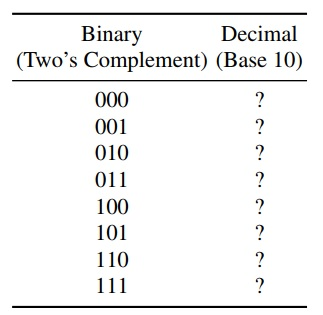
\includegraphics[width=0.5\linewidth]{figuras/exe_1-8}
\end{center}




\newpage
\section{Teste}

O estado quântico $\ket{\psi}$ é representado como um ket vector.

$\ket{0}$, $\ket{1}$

$\alpha_{1}, \alpha_{2}, \alpha_{3}$

\(\alpha_{4}, \alpha_{5}, \alpha_{6} \)

O conjunto dos números reais é denotado por $\mathbb{R}$.


% \lipsum[1-10]  % Exemplo de texto de preenchimento

\newpage
%Biblioteca
\bibliographystyle{unsrt} %estilo
\bibliography{./referencias/referencias}
	
\end{document}